\documentclass[titlepage]{jsarticle}
\usepackage[dvipdfmx]{graphicx}
\usepackage{listings}
\usepackage{h31ec-exp}
\lstset{
  basicstyle={\ttfamily},
  identifierstyle={\small},
  commentstyle={\smallitshape},
  keywordstyle={\small\bfseries},
  ndkeywordstyle={\small},
  stringstyle={\small\ttfamily},
  frame={tb},
  breaklines=true,
  columns=[l]{fullflexible},
  numbers=left,
  xrightmargin=0zw,
  xleftmargin=3zw,
  numberstyle={\scriptsize},
  stepnumber=1,
  numbersep=1zw,
  lineskip=-0.5ex
}
\renewcommand{\lstlistingname}{ソースコード}
\makeatletter
\newcommand{\figcaption}[1]{\def\@captype{figure}\caption{#1}}
\newcommand{\tblcaption}[1]{\def\@captype{table}\caption{#1}}
\makeatother
\title{オートマトンのプログラミング}
\grade{3年32番}
\author{平田 蓮}
\team{第4班}
\date{2019年11月19日}
\expdate{2019年11月6日, 11月11日, 11月18日}
\coauthor{
    4番  石橋那起 \\
    8番  小林歩夢 \\
    12番  小室弦太 \\
    15番  佐藤貴幸 \\
    20番  関晋一朗 \\
    24番 高橋祐己哉 \\
    28番 外川諒太郎 \\
    36番  本多充稔
}

\begin{document}
\maketitle
\section{目的}
    本実験では, Raspberry Piを用いてLinux環境を構築し, その手順とともにIoT(Internet of Things)システム開発の基礎を習得する.

\section{IoT(Internet of Thing)}
    オートマトンとは自動機械という意味であるが、工学で用いられる場合は、離散的な入力及び出力
    を持つ機械のモデルのことであり, 状態とその遷移という考え方で捉える.
    ある装置の動作を実現することを考えた場合に, 入出力をまず考えるが, それだけでは動作を実現することは
    できない. 出力を決定する要素として内部状態という考えが必要である.

    装置の取り得る内部状態の数が有限個の場合, その装置を有限オートマトンといい, その動作は次の5個の
    集合と関数で記述できる.

    \paragraph{FAに必要な集合と関数}
        上で述べた集合と関数を示す.

        \begin{itemize}
            \item $X$: 入力集合
            \item $Q$: 状態集合
            \item $Z$: 出力集合
            \item $\sigma$: 状態遷移関数 $\sigma(X, Q) \rightarrow Q$
            \item $\omega$: 出力関数 $\omega(X, Q) \rightarrow Z または \ \omega(Q) \rightarrow Z$
        \end{itemize}

    \subsection{状態遷移図}
        FAの動作を図で表すには状態遷移図を用いると良い.

        例として10円硬貨だけが使える30円切手自動販売機を考える.
        Cancelボタンを押すと払い戻しとする.

        \begin{itemize}
            \item $X$: \{10[円], Cancel\}
            \item $Q$: \{0[円], 10[円], 20[円]\} (初期状態: 0[円])
            \item $Z$: \{1[枚], 10[円], 20[円]\}
        \end{itemize}

        このFAの状態遷移図を図\ref{fig:例状態遷移図}に示す.
        以下, 全ての状態遷移図で入出力を入力/出力のように示す.

        \begin{figure}[ht]
            \centering
            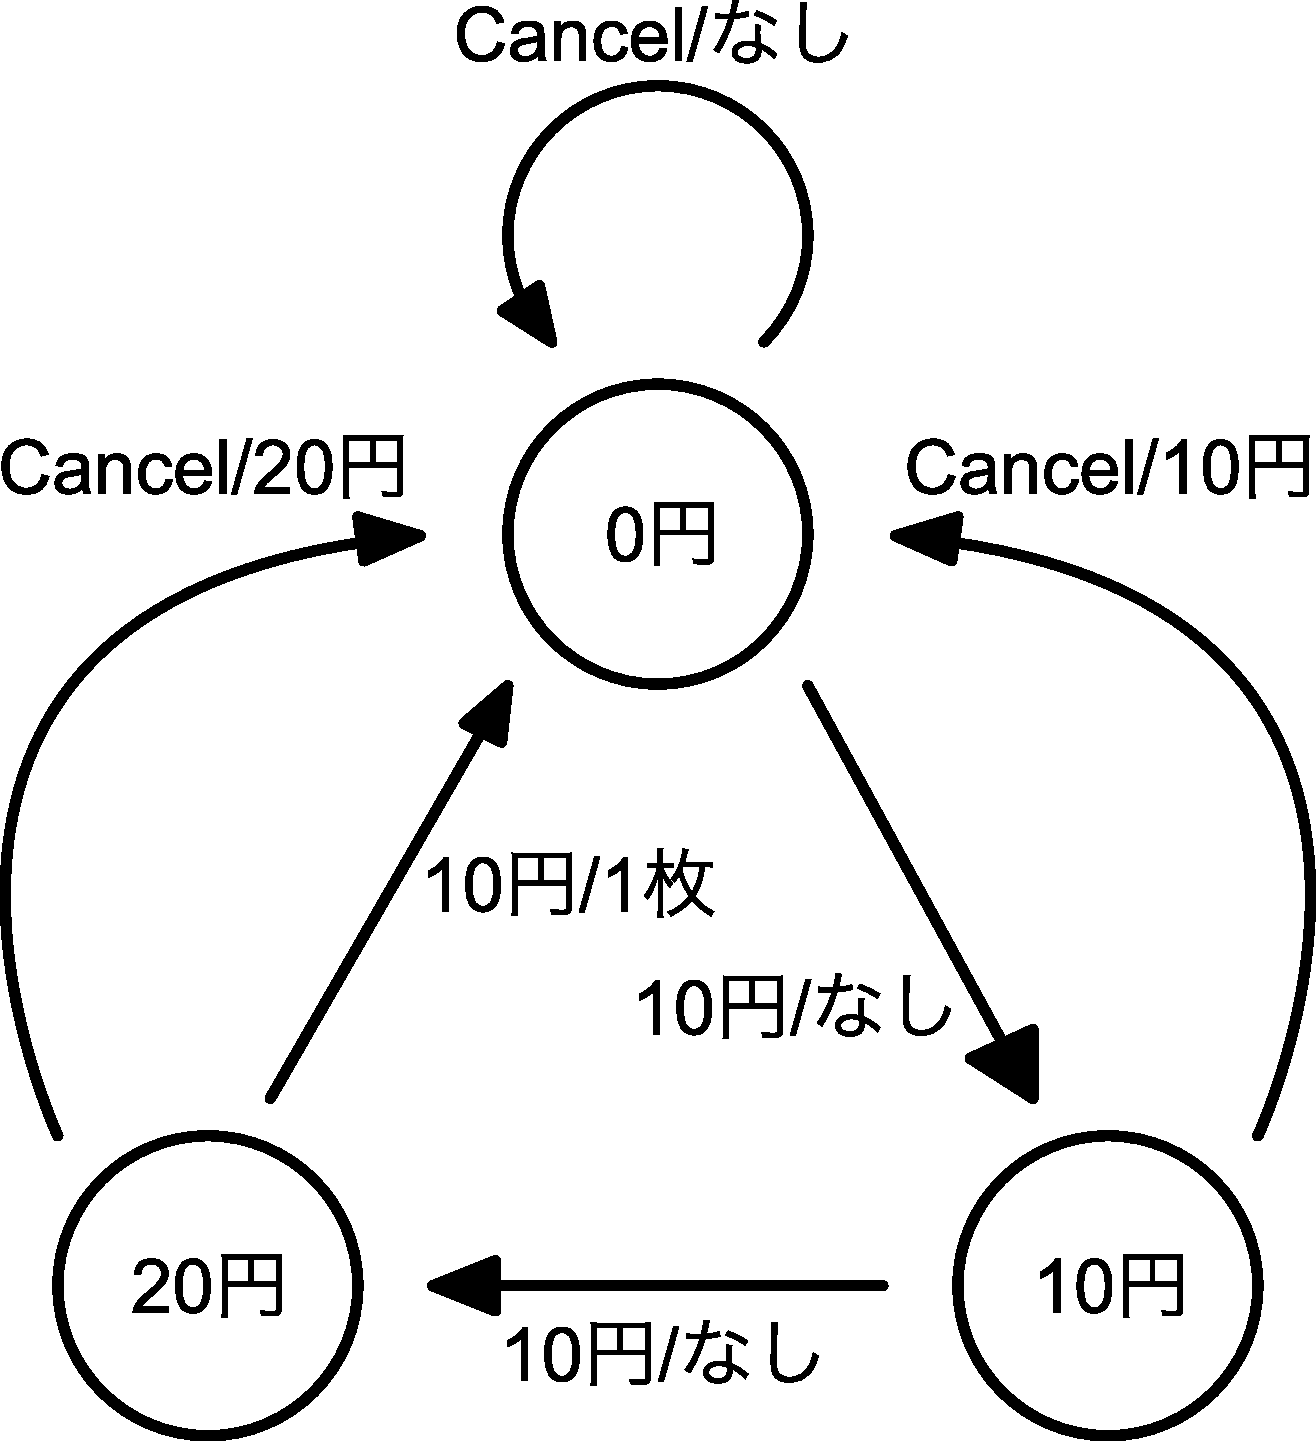
\includegraphics[width=8cm]{images/rei.pdf}
            \caption{30円切手自動販売機}
            \label{fig:例状態遷移図}
        \end{figure}

\section{練習問題}
    実験テキストの練習問題の状態遷移図を示す.

    (1) 10円硬貨だけが使用できる40円切手自動販売機. Cancelを押すと払い戻し.

    \begin{figure}[ht]
        \centering
        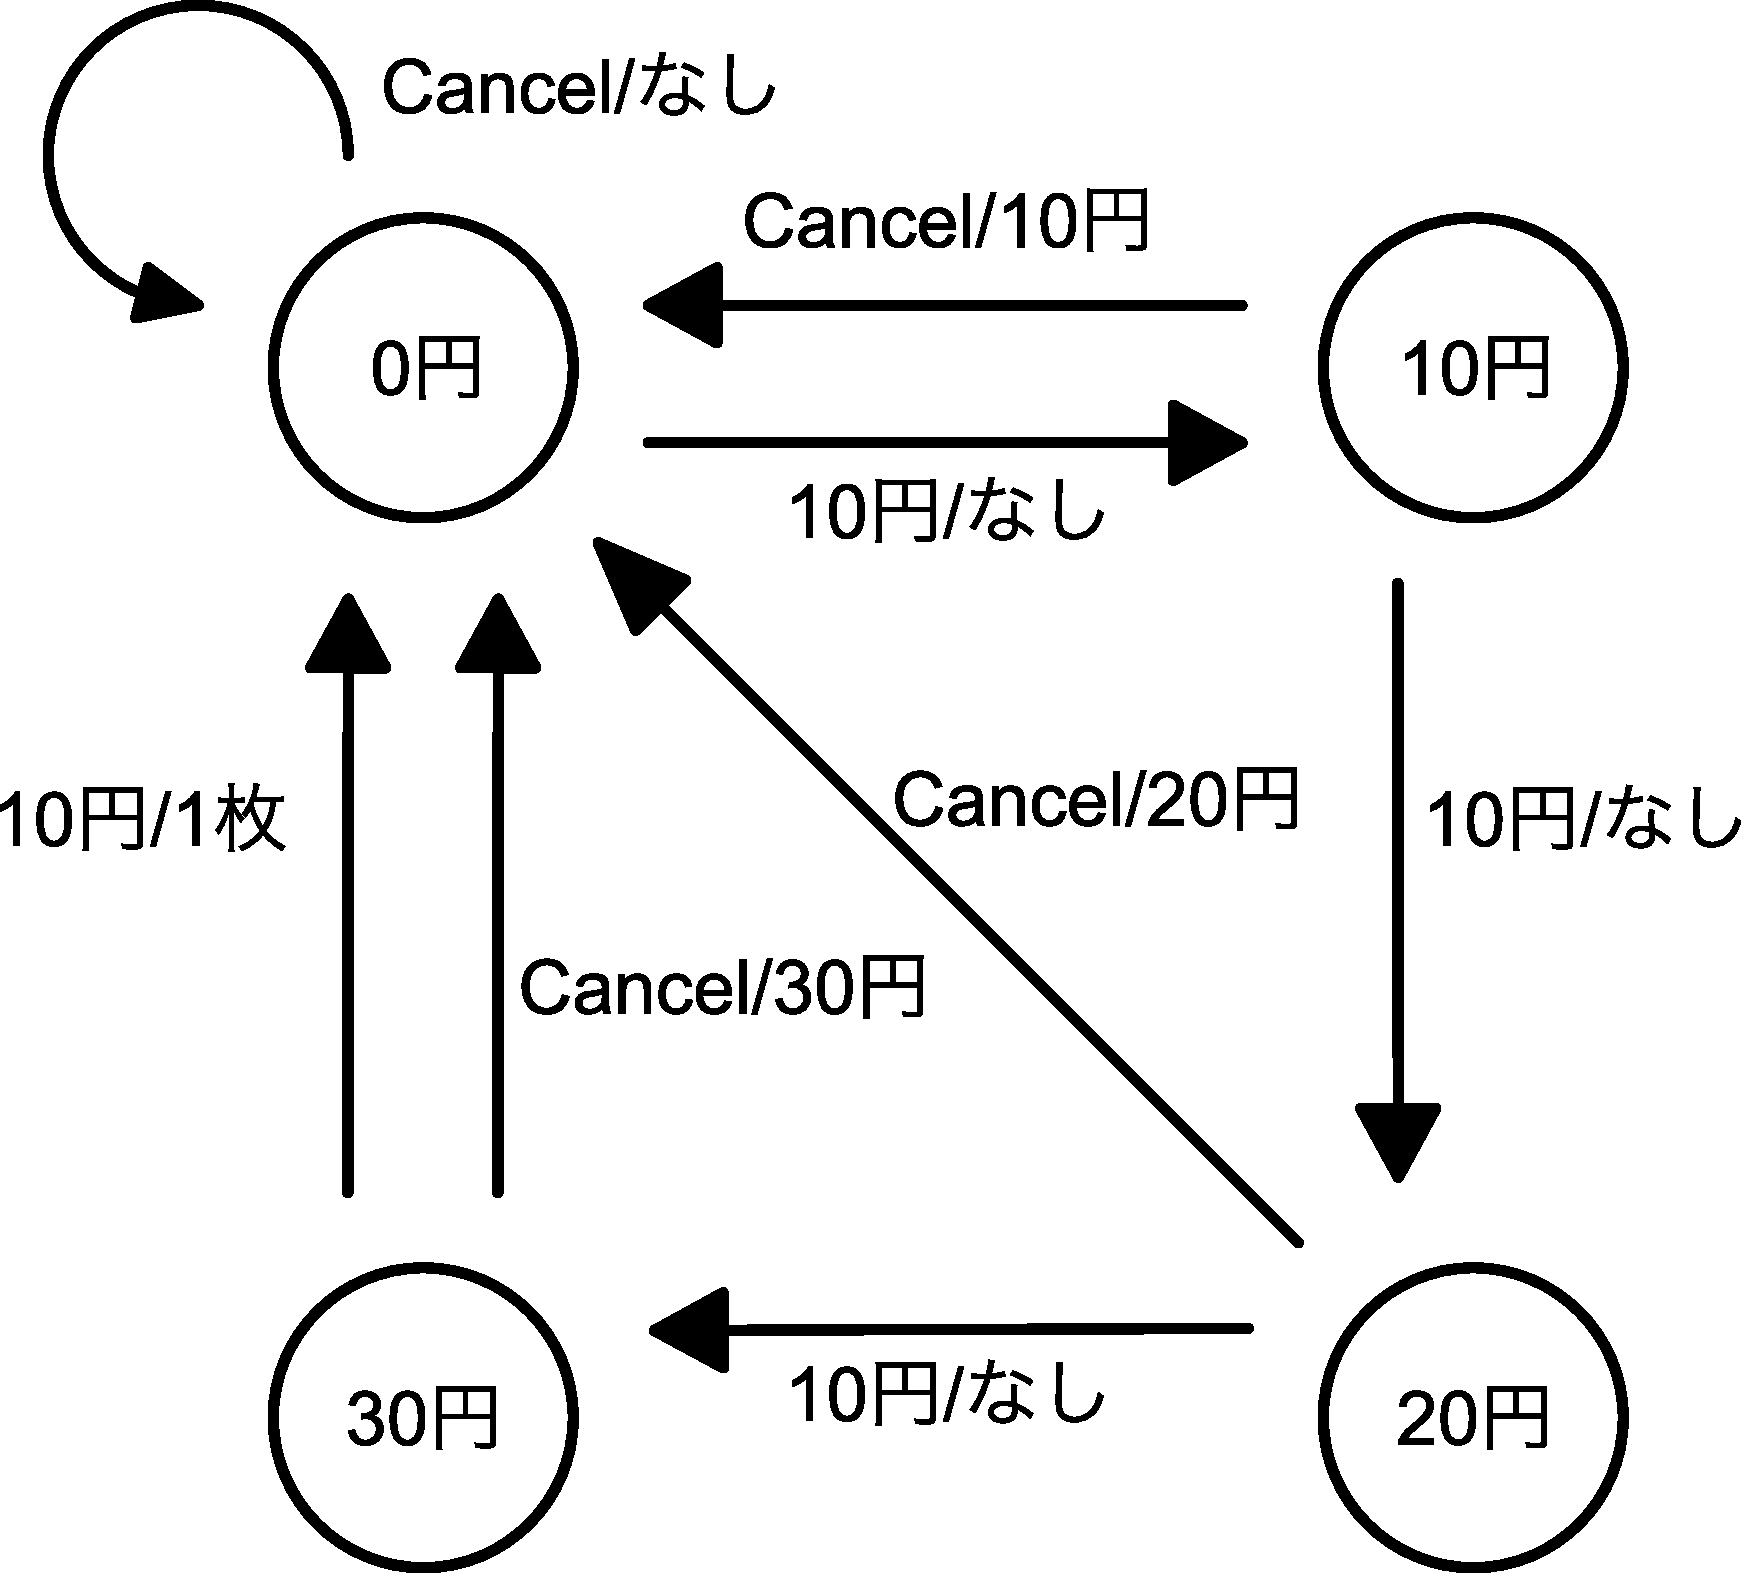
\includegraphics[width=8cm]{images/40.pdf}
        \caption{40円切手自動販売機}
        \label{fig:40状態遷移図}
    \end{figure}

    (2) 10円硬貨と50円硬貨だけ使える30円切手自動販売機. Cancelを押すと払い戻し.
    (お釣りはCancelを押さないと出てこない.)

    \begin{figure}[ht]
        \centering
        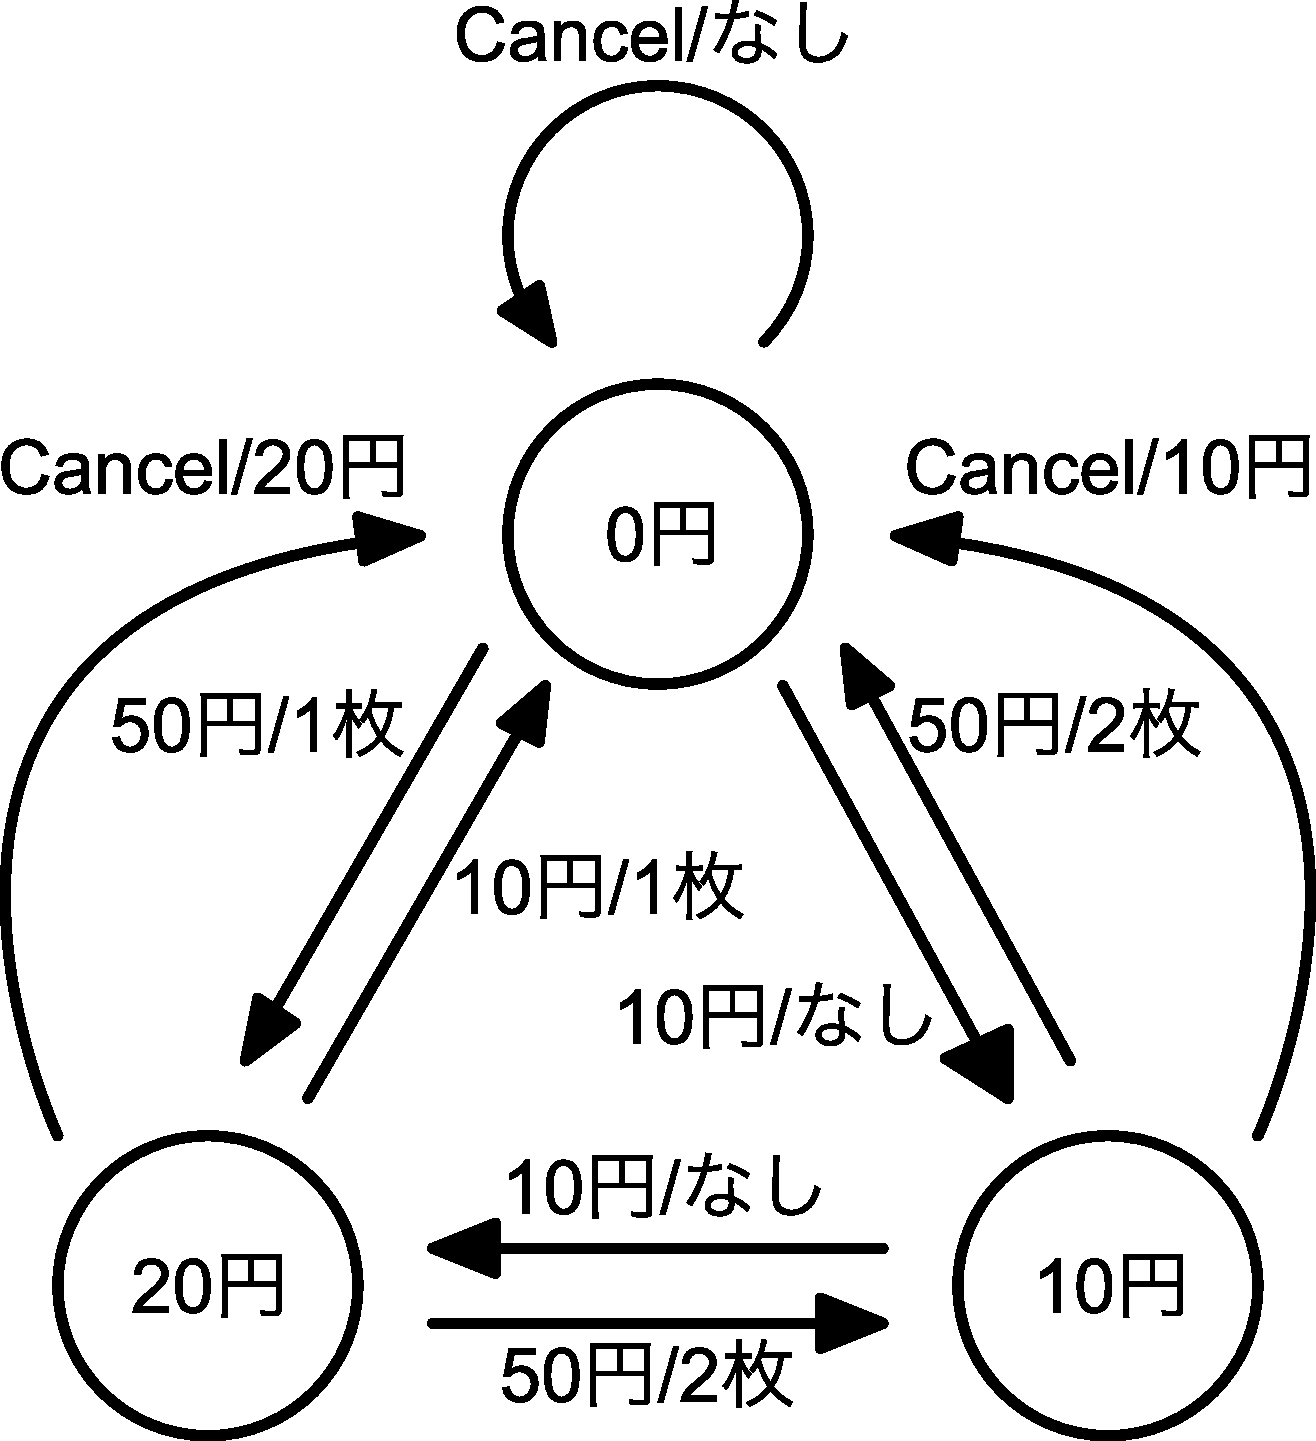
\includegraphics[width=8cm]{images/30.pdf}
        \caption{30円切手自動販売機}
        \label{fig:30状態遷移図}
    \end{figure}

    (3) 10円, 50円, 100円硬貨が使える20円切手自動販売機. Cancelを押すと払い戻し.
    (お釣りはCancelを押さないと出てこない.)

    \begin{figure}[ht]
        \centering
        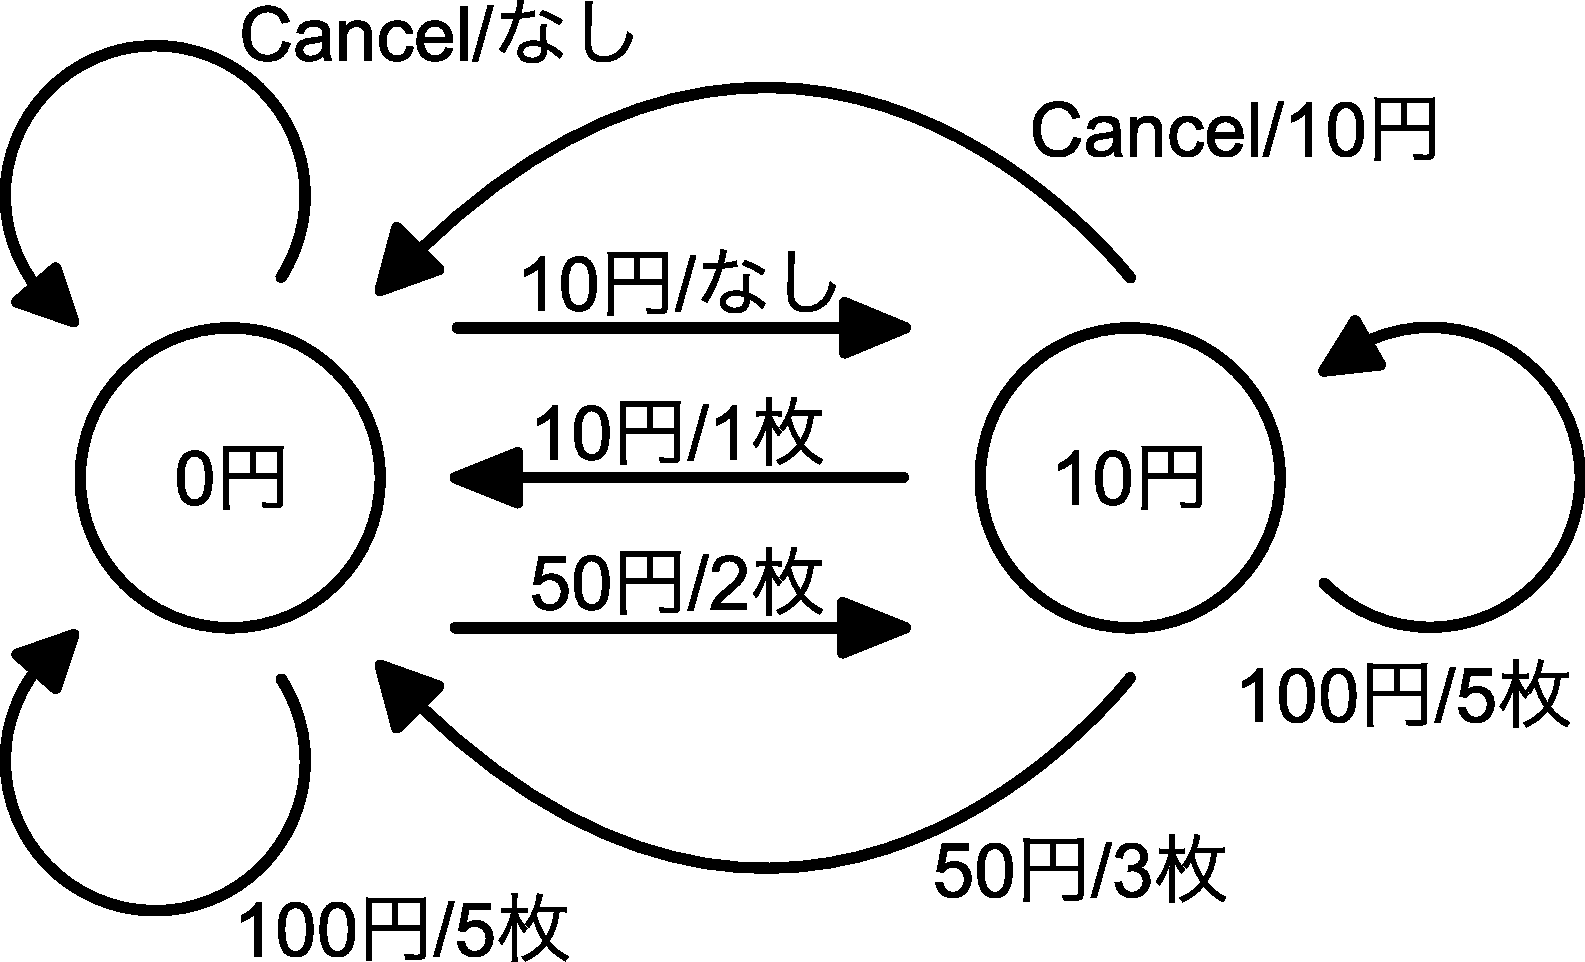
\includegraphics[width=8cm]{images/20.pdf}
        \caption{20円切手自動販売機}
        \label{fig:20状態遷移図}
    \end{figure}

\section{仮想自動販売機作成実習}
    今回は, 10円と50円が使える20円切手自販機を実装してみた.
    10円入ってるときに50円を入れると60円になり切手が3枚出力されるので,
    3枚目は100円のランプを使うこととする.
    また, Cancelを押すと払い戻しをする.

    図\ref{fig:本番状態遷移図}に状態遷移図を示す.

    \begin{figure}[ht]
        \centering
        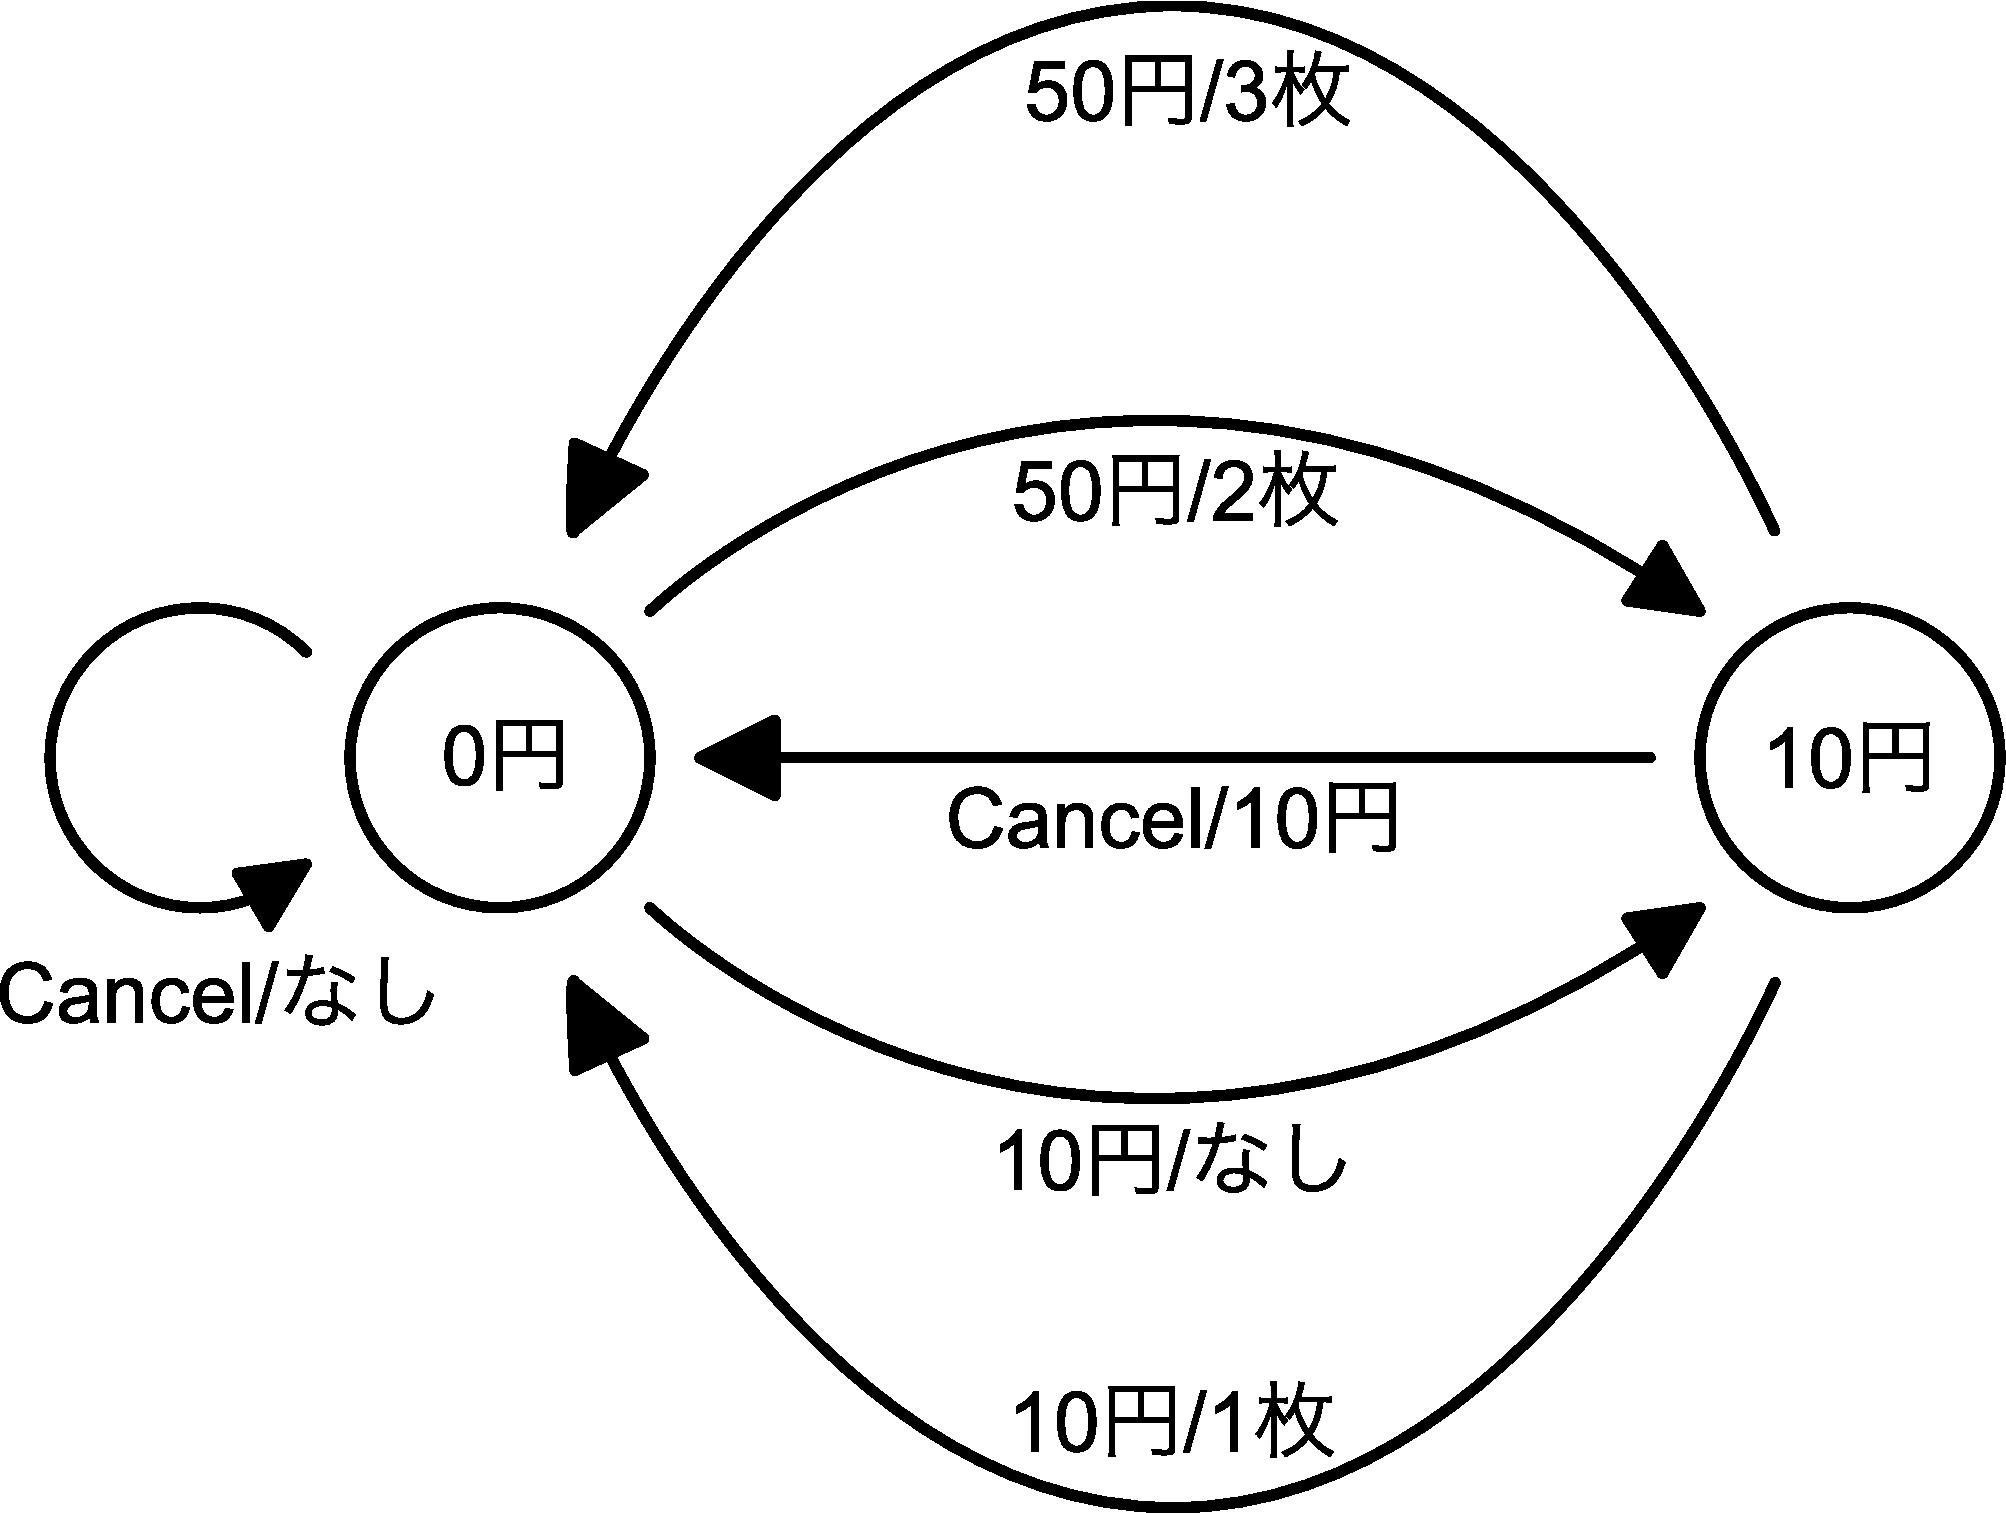
\includegraphics[width=8cm]{images/honban.pdf}
        \caption{20円切手自動販売機状態遷移図}
        \label{fig:本番状態遷移図}
    \end{figure}

    \subsection{ソースコード}
        今回変更を加えた部分のソースコードを以下に示す. \\

        \begin{lstlisting}[caption=piclib.c, label=piclib]
void  StampOut(int num) {
    if (num > 2) led_on(LED100);
    if (num > 1) led_on(STAMP2);
    if (num > 0) led_on(STAMP1);
}
        \end{lstlisting}

        \begin{lstlisting}[caption=piclib.h extern.h]
void StampOut(int num);		/* スタンプ表示		*/
        \end{lstlisting}

        \begin{lstlisting}[caption=stamp.c 遷移関数, label=transition]
int Transition (char it, Status* st, int* a, int* b) {
    *a = *b = 0;	/* コインA,Bの出力枚数を0にしておく */
    if (it == Exit) *st = stExit;
    if (it == Cancel) {
        *a = *st;
        *st = stEmpty;
    }
    if (it == CoinA) {
        ++*st;
        *st = *st % 2;
        if (!*st) {
            return 1;
        } else {
            return 0;
        }
    }
    if (it == CoinB) {
        *st += 5;
        *st = *st % 2;
        if (*st) {
            return 2;
        } else {
            return 3;
        }
    }
    return 0;
}
        \end{lstlisting}

        \begin{lstlisting}[caption=stamp.c メインループ, label=main]
do {
    it = sw_read();
    if (it == 0) continue;
    outfg = outcoin = 0;
    s = Transition(it, &st, &a, &b);
    DispStatus(status_bit[st]);
    if (a | b) outfg = 1;
    StampOut(s);
    if (a) DispCoinA(a);
    if (b) DispCoinB(b);
    while(it = sw_read()){	/*  スイッチ入力監視	*/
        if (it == Exit) break;
        timer(30);
    }
} while (st != stExit);
        \end{lstlisting}

        まず, ソースコード\ref{piclib}にあるように, 切手の出力をする関数を複数枚出力ができるように変更した.
        StanpOut関数は引数で切手の枚数を受け取り, その値の個数だけLEDを光らせる.
        また, それに伴いpiclib.hとextern.hにあるStampout関数のプロトタイプ宣言を変更した.

        ソースコード\ref{transition}には, 変更後の遷移関数を示した.
        遷移関数Transitionは受け付ける入力を2種類に増やし,
        それぞれの入力に対し適切な切手枚数を返すように変更した.

        最後に, これらの変更に伴い, ソースコード\ref{main}のようにstamp.cのメインループ内を変更した.
    
\section{調査課題「ワンチップマイコンについて調査せよ」}
    コンピュータを形成するのに必要な要素は入出力装置, 記憶装置, 処理装置などである.
    これらを一つのICにまとめたものがワンチップマイコンである.

    ワンチップマイコンの特徴として, 以下のものが挙げられる.

    \begin{itemize}
        \item 小さい
        \item 安い
        \item 多種類
        \item プログラムの書き換えが可能
    \end{itemize}

    現在主流のワンチップマイコンは, Microchip社製のPICシリーズと,
    現在はMicrochip社に買収されたAtmel社製のAVRシリーズがある.
    今回の実験ではPICシリーズを使用した.

    AVRにはPICと比べて以下のような特徴がある.

    \begin{itemize}
        \item 高速
        \item 操作が簡単
        \item 知名度が低く, 情報が少ない
    \end{itemize}

    それぞれに特徴があり, 用途によって使い分けることが必要である.

\section{考察}
    

\section{感想}


\begin{thebibliography}{99}
    \bibitem{IoT} IoTとは? MONO WIRELESS https://mono-wireless.com/jp/tech/Internet\_of\_Things.html
\end{thebibliography}

\end{document}
